\begin{frame}{Working With Cumulative Probabilities}
    Practice rewriting the following probabilities in terms of $P(X \le x)$ and $P(X=x_1)+P(X=x_2)+\dots$.
    \begin{itemize}
        \item $P(X < 4)$
        \item $P(X > 4)$
        \item $P(X \le 4)$
        \item $P(X \ge 4)$
    \end{itemize}
\end{frame}

\begin{frame}{Working With Cumulative Probabilities}
    Practice rewriting the following probabilities in terms of $P(X \le x)$ and $P(X=x_1)+P(X=x_2)+\dots$.
    \begin{itemize}
        \item $P(6 \le X \le 8)$
        \item $P(6 \le X < 8)$
        \item $P(6 < X \le 8)$
        \item $P(6 < X < 8)$
    \end{itemize}
\end{frame}

\begin{frame}{Motivating Example: Poisson Distribution}
    \begin{itemize}
        \item There are about 8 million people in New York City.
        \item How many New Yorkers would be expect to be hospitalized due to heat attack, each day?
        \item Historical records suggest the average is 4.4
        \item But what about the distribution? 
        \item What might a histogram of daily counts look like?
    \end{itemize}
\end{frame}

\begin{frame}{Example}
    Intuitively, we might think that
    \begin{itemize}
        \item The average is 4.4.
        \item We don't know the standard deviation.
        \item The minimum is 0.
        \item The (theoretical) maximum is about 800 million or so. It's so far away from the mean as to be meaningless.
    \end{itemize}
    Clearly the maximum is a lot further from the average than the minimum is, so we might guess that this distribution is skewed to the right.
\end{frame}

\begin{frame}{Example}
    \begin{center}
        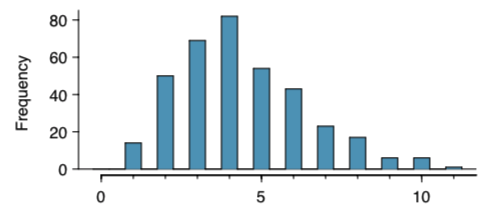
\includegraphics[scale=.4]{images/poisson1.png}
    \end{center}
    \vspace{-10pt}The number of heart attack hospitalizations were recorded every day for a year.
    \begin{itemize}
        \item The sample mean is 4.38, similar to the historical average of 4.4.
        \item The sample standard deviation is about 2.
        \item The distribution is unimodal and right-skewed.
    \end{itemize}
\end{frame}

\begin{frame}{The Poisson Distribution}
    The \textbf{Poisson distribution} is used to describe the number of events that occur in a large population over some period of time. We might measure
    \begin{itemize}
        \item Marriages
        \item Births
        \item Heart attacks
        \item Lightning strikes
    \end{itemize}
    In each case, we can count the number of times that event occurs during a period of time. 
\end{frame}

\begin{frame}{The Poisson Distribution}
    \begin{itemize}
        \item The average number of occurrences per period of time is called the \textbf{rate}.
        \item In the heart attack example, we had a rate of 4.4 \textit{heart attacks} (the event) per \textit{day} (the period of time).
        \item We denote the rate by the Greek letters $\lambda$ (lambda) or $\mu$.
        \item We can use this information to find the probability of observing exactly $k$ events during a particular period of time.
    \end{itemize}
\end{frame}

\begin{frame}{The Poisson Distribution}
    Suppose we are interested in some events and the number of observed events follows a Poisson distribution with rate $\lambda$. Let $X$ be the number of events observed. Then
    \[
        P(X=k) = \frac{\lambda^k e^{-\lambda}}{k!}.
    \]
    where $k$ can take on any whole number greater than or equal to 0. The letter $e$ is a constant: $e\approx 2.719$.
\end{frame}

\begin{frame}{The Poisson Distribution}
    The Poisson distribution has an interesting property: its mean and variance are the same!
    
    \[
    E(X) = Var(X) = \lambda
    \]
    
    and the standard deviation is then $\sqrt{\lambda}$.
\end{frame}

\begin{frame}{Is It Poisson?}
    Guidelines for determining if the Poisson distribution is appropriate:
    \begin{enumerate}
        \item We are interested in the number of events that occur.
        \item There is a set period of time that we are interested in.
        \item Events occur independently of each other.
        \item The population that generates the events is quite large.
    \end{enumerate}
\end{frame}

\begin{frame}{Example: Coffee Shop Customers}
    A coffee shop serves an average of 75 customers per hour during the morning rush.
    \begin{itemize}
        \item Which distribution is appropriate for working with the probability of a given number of customers arriving within one hour during the morning rush?
    \end{itemize}
\end{frame}

\begin{frame}{Example: Coffee Shop Customers}
    \begin{enumerate}
        \item We are interested in the number of customers served.
        \begin{itemize}
            \item "Customer served" is the event.
        \end{itemize}
        \item We are interested in this event over the course of one hour (during morning rush), so there is a set period of time.
        \item We assume that customers are served (more or less) independently of one another.
        \item The population that generates these events is anyone who could possibly walk in and be served during the morning rush. That's quite a lot of people, so can be confident that the population is large.
    \end{enumerate}
    So the Poisson distribution is appropriate.
\end{frame}

\begin{frame}{Example: Coffee Shop Customers}
    What are the mean and standard deviation of the number of customers this coffee shop serves in one hour during the morning rush?
\end{frame}

\begin{frame}{Example: Coffee Shop Customers}
    Would it be considered unusually low if only 60 customers showed up to the coffee shop in one hour during the morning rush?
\end{frame}

\begin{frame}{Example: Coffee Shop Customers}
    Find the probability that the coffee shop serves 70 people in one hour during the morning rush.
\end{frame}

\begin{frame}{Example: Coffee Shop Customers}
    What is the probability that the coffee shop serves between (and including) 73 and 76 customers?
\end{frame}

\begin{frame}{Poisson Approximation to Binomial}
    This is another binomial approximation method that will help us avoid difficult factorial expressions.
    
    \vspace{12pt}We can use the Poisson approximation to the binomial distribution when
    \begin{itemize}
        \item $n$ is large
        \item $np < 7$
    \end{itemize}
\end{frame}

\begin{frame}{Poisson Approximation to Binomial}
    Suppose we have a lot size of 1000 and the proportion of defective items is 0.001. What is the probability of exactly 3 defective items?
    \begin{itemize}
        \item Items are either defective or not.
        \item Defective status is independent between items.
        \item There is a fixed lot size of $n=1000$ items.
        \item The probability of success (a defect) is 0.001.
    \end{itemize}
\end{frame}

\begin{frame}{}
    The binomial probability for exactly 3 defectives is
    \begin{align*}
        P(X=3) &= {1000 \choose 3}(0.001)^3(0.999)^{1000-3} \\
        &= 0.0613
    \end{align*}
    OR, we can let $\lambda=np=1$ and use the Poisson distribution:
    \begin{align*}
        P(X=3) &= \frac{e^{-1}1^3}{3!} \\
        &= 0.0613
    \end{align*}
\end{frame}